\section{Appendici}
\appendix
\section{ISO/IEC 15504}
Lo standard ISO/IEC 15504, comunemente chiamato SPICE* (acronimo di Software Process Improvement and Capability Determination), viene utilizzato per eseguire una valutazione concreta della qualità dei processi, inoltre permette la misurazione della capability dei processi, ovvero la maturità di un processo l'abilità con cui esso raggiunge l'obiettivo. Per eseguire queste misurazioni lo standard offre nove attributi da associare ai processi, ognuno dei quali misura un particolare aspetto della maturità del processo:
	\begin{itemize}
	\item \textbf{Process performance:} è una misura del grado con cui è stato raggiunto lo scopo del processo
	\item \textbf{Perfomance management:} è una misura del grado con il quale la performance del processo viene gestita
	\item \textbf{Work product management:} è una misura del grado con il quale i risultati prodotti dal processo vengono appropriatamente gestiti
	\item \textbf{Process definition:} è una misura del grado con cui uno standard di processo è mantenuto (utilizzato) a supporto dell'implementazione del processo.
	\item \textbf{Process deployment:} è una misura del grado con il quale lo standard di processo viene effettivamente distribuito come un processo definito in grado di raggiungere gli obiettivi del processo stesso.
	\item \textbf{Process measurement:} è una misura del grado con il quale i risultati delle misurazioni sono utilizzati per garantire che le prestazioni del processo supportino il raggiungimento degli obiettivi di prestazione pertinenti del processo a sostegno di determinati obiettivi di business.
	\item \textbf{Process control:} è una misura del grado con il quale il processo è quantitativamente gestito per produrre un processo che sia stabile, abile e previdibile entro limiti definiti.
	\item \textbf{Process innovation:} è una misura del grado con il quale vengono identificate delle modifiche al processo attraverso l'analisi di cause comuni di variazione delle performance, e dalla ricerca di approcci innovativi alla definizione e all'implementazione del processo.
	\item \textbf{Process optimization:} è una misura del grado con il quale delle modifiche alla definizione, gestione e alle prestazioni del processo si traducono in un impatto che porta a raggiungere rilevanti miglioramenti al processo.
	\end{itemize}
	A questi attributi viene assegnato uno dei seguenti quattro livelli di misura:
	\begin{itemize}
	\item \textbf{N not implemented:} non ci sono segni di raggiungimento dell'attributo.
	\item \textbf{P partial implemented:} esistono alcuni risultati dell'attributo in questione.
	\item \textbf{L largely implemented:} ci sono significanti segni di raggiungimento dell'attributo in questione.
	\item \textbf{F fully implemented:} viene identificato un pieno raggiungimento degli obiettvi dell'attributo
	\end{itemize}
	Infine sulla base delle valutazioni assegnate ad ogni attributo del processo, potrà essere valutato il grado complessivo di maturazione, il quale varierà sui seguenti sei valori:
	\begin{itemize}
	\item \textbf{0 - Incomplete:} viene rilevato un fallimento generale nel conseguimento dell'obiettivo del processo. Non si identifica alcun prodotto o risultato. Un processo appartenente a questo livello non può essere associato ad alcun attributo.
	\item \textbf{1 - Performed:} lo scopo del processo è generalmente raggiunto, a prova di ciò sono identificabili dei prodotti risultanti dal processo. A questo livello il processo viene associato all' attributo Process performance.
	\item \textbf{2 - Managed:} il processo raggiunge dei risultati di qualità accettabile rispettando i tempi prestabiliti. Il risultato soddisfa tutti i requisiti e gli standard predefiniti. Un processo a questo livello è quindi gestito tramite pianificazione e controllo e correzione dei suoi risultati, i quali possono essere ritenuti sicuri. Gli attributi associati a questo livello sono process management e work product management.
	\item \textbf{3 - Estabilished:} il processo è implementato, gestito mediante procedure ben definite basate sui buoni principi dell'ingegneria del software*. Un processo appartenente a questo livello sarà in grado di raggiungere sempre gli stessi risultati. Process definition e process distribution sono gli attributi associabili a questo livello.
	\item \textbf{4 - Predictable:} il processo raggiunge i propri obiettivi all'interno di limiti di controllo definiti. La sostanziale differenza con il livello estabilished è che ora il processo è quantitativamente compreso e controllato. A questo livello vengono associati gli attributi process measurement e process control.
	\item \textbf{5 - Optimizing:} le attività del processo sono ottimizzate per affrontare bisogni progettuali presenti e futuri, il processo viene sottoposto a miglioramento continuo. Gli attributi associati a questo livello sono process innovation e process optimization.
	\end{itemize}
	\begin{figure}[htbp]
	\centering
	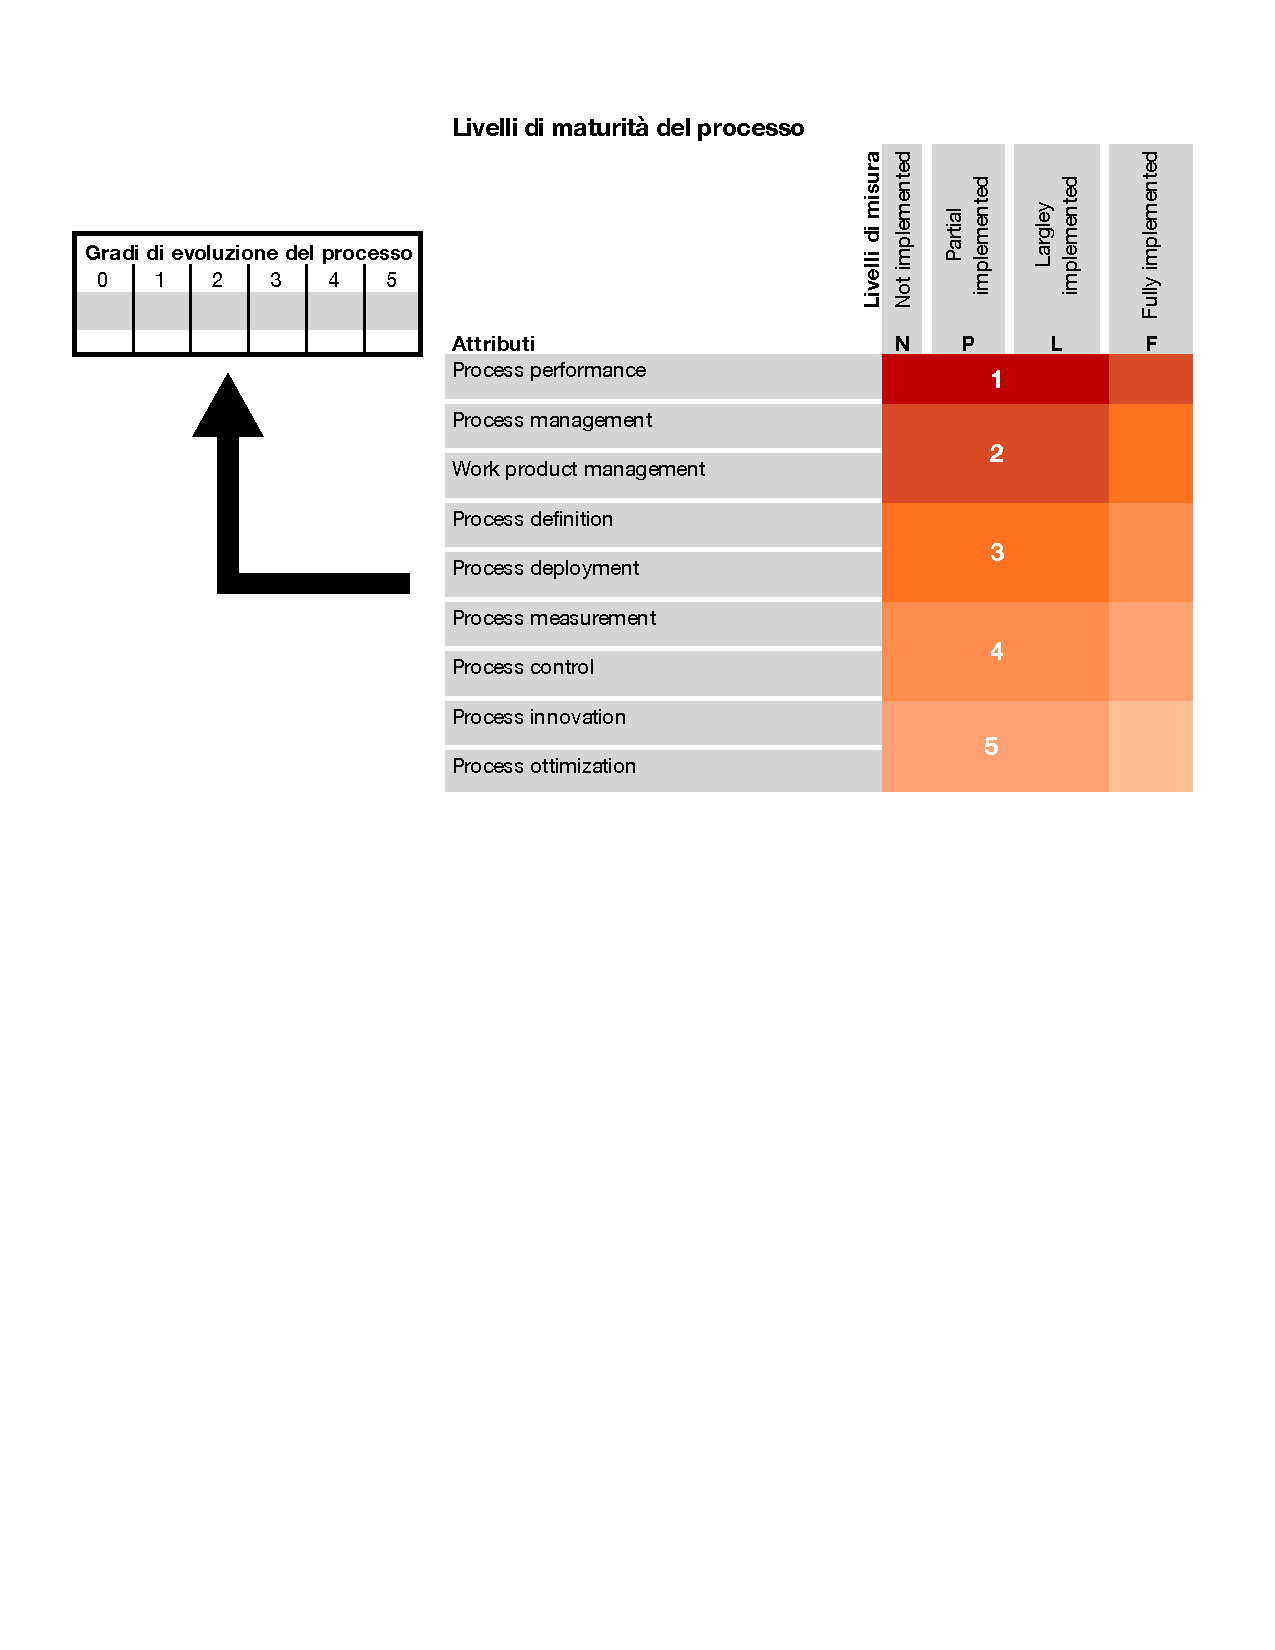
\includegraphics[scale=0.7]{images/ISOIEC15504.pdf}
	\caption{Riepilogo modello ISO/IEC 15504}
	\end{figure}
\section{ISO/IEC 9126}
Lo standard ISO/IEC 9126 definisce un modello dei requisiti qualitativi del Prodotto.
	  Il modello descritto si concentra in primo luogo sui tre punti di vista della qualità che esistono sul prodotto:
	  \begin{itemize}
	  \item \textbf{Qualità esterna:} esprime il comportamento dinamico del software, in un determinato ambiente d'uso. In sostanza consiste nelle prestazioni e nelle funzionalità che il prodotto offre quando è in esecuzione;
	  \item \textbf{Qualità interna:} esprime le proprietà statiche, cioè
indipendenti dal contesto di esecuzione e uso. Sono direttamente misurabili ad esempio sul
codice sorgente, pertanto senza la necessità di eseguire il software;
	  \item \textbf{Qualità in uso:} esprime il livello con cui il prodotto si dimostra utile all'utente nel suo contesto d'uso. In altre parole rappresenta la capacità del prodotto di dare efficacia ed efficienza al lavoro dell'utente, a fronte di una sicurezza di utilizzo e di una soddisfazione nel far uso del prodotto.
	  \end{itemize}
	  \subsubsection{Modello per la qualità esterna ed interna}
	  Per la qualità esterna ed interna è definito un modello gerarchico formato da 6 caratteristiche principali e numerose sottocaratteristiche, tutte misurabili direttamente o indirettamente grazie all'utilizzo di metriche.
	  Le sei caratteristiche principali sono elencate di seguito:
	  \begin{itemize}
	  \item \textbf{Funzionalità:} rappresenta la capacità del prodotto software di fornire funzioni che soddisfano le esigenze stabilite, sia esplicite che implicite, quando il software opera in un determinato contesto di utilizzo. Sottocaratteristiche notevoli sono l'interoperabilità e la Sicurezza, intesa come la capacità di proteggere le informazioni e i dati da accessi non autorizzati;
	  \item \textbf{Affidabilità:} capacità di mantenere uno specificato livello di prestazione quando si opera in specificate condizioni. Sottocaratteristiche importanti sono la maturità e la tolleranza all'errore;
	  \item \textbf{Efficienza:} capacità di fornire le funzioni richieste nel minor tempo possibile, sfruttando al meglio le risorse messe a disposizione;
	  \item \textbf{Usabilità:} capacità del prodotto software di essere capito, appreso, usato e gradito all'utente, quando usato in contesti specificati. Una sottocaratteristica di rilievo è l'attrattiva;
	  \item \textbf{Manutenibilità:} capacità del software di essere modificato e manutenuto. Per modifiche si intendono correzioni o adattamenti del software, negli ambienti, nei requisiti e nelle specifiche funzionali. Una sottocaratteristica importante è la testabilità, cioè la capacità di un software di consentire la verifica e di essere oggetto di test;
	  \item \textbf{Portabilità:} capacità di poter essere trasferito da un ambiente di esecuzione all'altro.
	  \end{itemize}
	  \subsubsection{Modello per la qualità in uso}
	  Per la qualità in uso lo standard definisce una gerarchia separata, per enfatizzare il fatto che qui si considera non solo il prodotto software in sè, ma la relazione stretta tra esso e l'utente, nell'ambiente di utilizzo. Il modello è formato dalle seguenti quattro caratteristiche:
	  \begin{itemize}
	  \item \textbf{Efficacia:} rappresenta la capacità di supportare un utente nel raggiungere i suoi obiettivi con accuratezza e completezza in un dato contesto;
	  \item \textbf{Produttività:} la capacità di supportare un utente nello spendere l’appropriata quantità di risorse in relazione all’efficacia dei risultati da raggiungere; 
	  \item \textbf{Soddisfazione:} la capacità di soddisfare un utente in un dato contesto d’uso;
	  \item \textbf{Safety:} la capacità di raggiungere accettabili livelli di rischio di
danni a persone, al software, ad apparecchiature, o all’ambiente operativo in un dato contesto d’uso.
	\end{itemize}
	\begin{figure}[htbp]
		\centering
		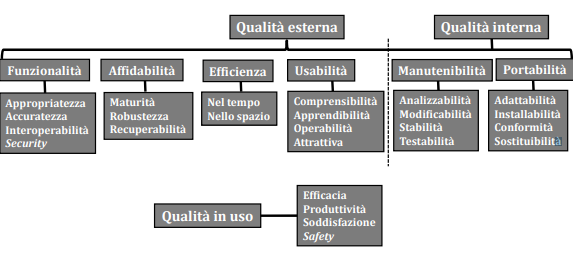
\includegraphics{images/gerarchiaQualitaProdotto.png}
		\caption{Riepilogo modello ISO 9126}
	\end{figure}